\documentclass[11pt]{article}
\usepackage[margin=.72in]{geometry}
\usepackage{amsmath,amssymb,lmodern,microtype,tikz,tcolorbox,fancyhdr,xcolor,needspace}
\usetikzlibrary{arrows.meta,patterns}
\tcbuselibrary{breakable}
\definecolor{navy}{RGB}{27,57,95}\definecolor{blue}{RGB}{47,117,181}\definecolor{amber}{RGB}{178,91,0}
\setlength{\parindent}{0pt}\setlength{\parskip}{9pt}\setlength{\jot}{14pt}
\pagestyle{fancy}\fancyhf{}\fancyhead[L]{Electricity \& Magnetism I}\fancyhead[R]{Lesson 14}\fancyfoot[C]{\thepage}\setlength{\headheight}{15pt}
\newcommand{\heading}[2]{\begin{center}{\LARGE\bfseries\color{navy} #1}\\[5pt]{\large #2}\end{center}\vspace{2pt}\hrule\vspace{9pt}}
\newcommand{\topic}[1]{\Needspace{12\baselineskip}\par{\Large\bfseries\color{navy}#1}\par}
\newcommand{\q}[2]{\par\bigskip\noindent\textbf{\color{navy}#1}\par\smallskip #2\par\medskip}
\newcommand{\work}[1]{\par\begin{center}\begin{tikzpicture}\draw[gray!45] (0,0) rectangle (15.3,{0.95*#1});\end{tikzpicture}\end{center}}
\newcommand{\concept}[2]{\begin{tcolorbox}[colback=blue!7,colframe=blue,title=#1,fonttitle=\bfseries,boxrule=.6pt,breakable]#2\end{tcolorbox}}
\newcommand{\coach}[1]{\begin{tcolorbox}[colback=blue!3,colframe=blue!55,title=Guided starting point,fonttitle=\bfseries,boxrule=.5pt,breakable]#1\end{tcolorbox}}
\newcommand{\route}[1]{\begin{tcolorbox}[colback=yellow!5,colframe=amber,title=Where this fits,fonttitle=\bfseries,boxrule=.5pt,breakable]#1\end{tcolorbox}}
\newcommand{\pausecheck}[1]{\begin{tcolorbox}[colback=white,colframe=navy!65,title=Check your thinking,fonttitle=\bfseries,boxrule=.5pt,breakable]#1\end{tcolorbox}}
\newcommand{\bridge}[1]{\begin{tcolorbox}[colback=white,colframe=amber,title=Physical starting point,fonttitle=\bfseries,boxrule=.5pt,breakable]#1\end{tcolorbox}}
\newcommand{\stage}[1]{\par\smallskip\noindent\textbf{\color{blue}#1}\par\smallskip}
\newcommand{\connect}[1]{\begin{tcolorbox}[colback=blue!4,colframe=blue!45,title=Keep the thread,fonttitle=\bfseries,boxrule=.45pt,breakable]#1\end{tcolorbox}}


\newcommand{\dipfig}{\begin{center}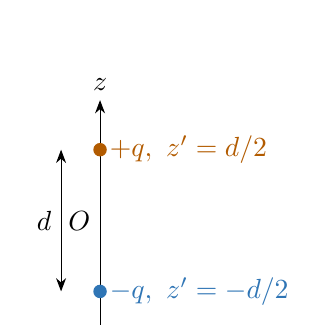
\begin{tikzpicture}[>=Stealth,scale=.9]
\draw[->] (0,-1.65)--(0,1.7) node[above] {$z$};
\fill[amber] (0,1) circle (.095) node[right] {$+q,\ z'=d/2$};
\fill[blue] (0,-1) circle (.095) node[right] {$-q,\ z'=-d/2$};
\node[left] at (0,0) {$O$};\draw[<->] (-.55,-1)--(-.55,1) node[midway,left] {$d$};
\end{tikzpicture}\end{center}}
\newcommand{\ringfig}{\begin{center}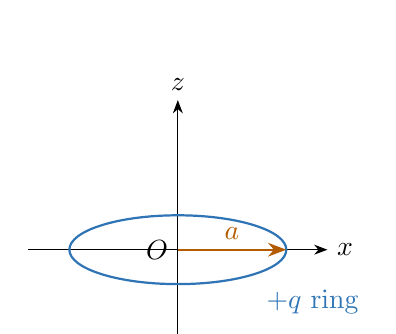
\begin{tikzpicture}[>=Stealth,scale=.95]
\draw[->] (0,-1.3)--(0,2) node[above] {$z$};
\draw[->] (-2,0)--(2,0) node[right] {$x$};
\draw[blue,thick] (0,0) ellipse (1.45 and .46);
\draw[->,amber,thick] (0,0)--(1.45,0) node[midway,above] {$a$};
\node[blue] at (1.8,-.7) {$+q$ ring};\node[left] at (0,0) {$O$};
\end{tikzpicture}\end{center}}
\newcommand{\linefig}{\begin{center}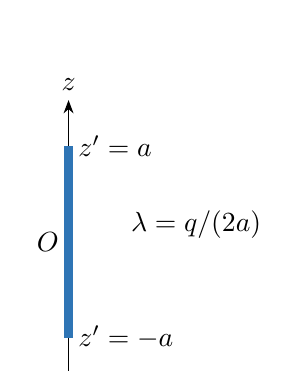
\begin{tikzpicture}[>=Stealth,scale=.9]
\draw[->] (0,-2)--(0,2) node[above] {$z$};
\draw[blue,line width=3pt] (0,-1.35)--(0,1.35);
\node[right] at (0,1.35) {$z'=a$};\node[right] at (0,-1.35) {$z'=-a$};
\node[left] at (0,0) {$O$};\node at (1.8,.25) {$\lambda=q/(2a)$};
\end{tikzpicture}\end{center}}
\begin{document}
\heading{Multipole Expansion: Five Charge Distributions}{Student Workbook — Guided Mathematical Development}
Name: \rule{7cm}{.3pt}\hfill Date: \rule{3cm}{.3pt}
\concept{What you will learn}{Recognize source geometry, choose the correct charge element, use symmetry to predict vanishing moments, evaluate the remaining moments, and interpret the far-field potential. Work with the Lesson 14 review guide open.}
\concept{Coordinate and notation reminder}{As in the lecture, $\theta$ is the polar angle from $+z$ and $\phi$ is azimuth. Your preferred convention reverses these symbols. A prime marks source coordinates, not a derivative.}
\concept{Useful Legendre values}{$P_0(x)=1$, $P_1(x)=x$, $P_2(x)=(3x^2-1)/2$, $P_3(x)=(5x^3-3x)/2$, $P_4(x)=(35x^4-30x^2+3)/8$. Also $P_n(1)=1$ and $P_n(-1)=(-1)^n$.}
\topic{Activity 1: Choose the correct multipole setup}
\route{Every example begins with source geometry, the charge element, and the convergence region. The index $n$ labels angular patterns, not individual charges.}

\q{1a.}{Explain the meaning of $r$, $r^\prime$, $\theta^\prime$, $dQ$, $Q_n$, and $R_{\max}$. Write the moment formula and the first three terms of the potential.}
\coach{Distinguish a small piece of physical charge $dQ$ from its weighted moment $Q_n$.}
\work{3}

\q{1b.}{Match each source to its charge element: point charges, a line, a ring, and a spherical cloud. Explain how to check normalization.}
\coach{For a ring $d\ell^\prime=a\,d\phi^\prime$; for a cloud $d\tau^\prime=r^{\prime2}\sin\theta^\prime dr^\prime d\theta^\prime d\phi^\prime$.}
\work{3}

\q{1c.}{Predict which moments vanish for a distribution unchanged under $z\mapsto-z$, and for one whose signed charge reverses under that reflection. Justify using $P_n(-x)=(-1)^nP_n(x)$.}
\coach{Pair source elements at opposite $z$ with the same $r^\prime$.}
\work{2.8}


\par\bigskip

\topic{Activity 2: A single point charge at the origin}
\route{Begin with the simplest source. This example also reveals why the multipole moments depend on the chosen origin.}

\q{2a.}{For a point charge $+q$ at the origin, identify $R_{\max}$ and evaluate $Q_0$ without a volume integral.}
\coach{Use the discrete-charge sum and $P_0=1$.}
\work{2.4}

\q{2b.}{Explain why every $Q_n$ with $n\ge1$ vanishes, even though the polar angle at the origin is undefined.}
\coach{The factor $r^{\prime n}P_n(\cos\theta^\prime)$ tends to zero as $r^\prime\to0$ for $n\ge1$.}
\work{2.6}

\q{2c.}{Write the complete exterior potential and check its angular dependence and domain. What changes if the coordinate origin moves?}
\coach{Only $Q_0$ survives for the centered charge.}
\work{2.7}


\par\bigskip

\topic{Activity 3: Two opposite charges on the polar axis}
\route{For the axial dipole, the charge signs and position signs both matter. Calculate the first moments explicitly before generalizing.}

\q{3a.}{Draw $+q$ at $z=d/2$ and $-q$ at $z=-d/2$. Label their radii and polar angles, then determine $R_{\max}$.}
\coach{Both source radii equal $d/2$, but their polar angles are $0$ and $\pi$.}
\work{2.6}

\q{3b.}{Calculate $Q_0$, $Q_1$, $Q_2$, and $Q_3$ separately, showing the contribution from each charge. Explain the parity pattern.}
\coach{Use $P_n(1)=1$ and $P_n(-1)=(-1)^n$.}
\work{3.4}

\q{3c.}{Write the first two nonzero potential terms. Identify the leading far-field term and explain its direction.}
\coach{The dipole moment points from the negative charge to the positive charge.}
\work{3}


\par\bigskip

\topic{Activity 4: A spherical charge cloud}
\route{The density $f(r^\prime)$ can vary radially. Spherical symmetry, not uniform density, removes the higher exterior moments.}

\q{4a.}{For $\rho=f(r^\prime)$ inside $r^\prime\le a$, write $dQ$, the integration limits, and the normalization equation for total charge $q$.}
\coach{The volume element contains $r^{\prime2}\sin\theta^\prime$.}
\work{3}

\q{4b.}{Factor the moment integral into radial and angular pieces. With $u=\cos\theta^\prime$, show why $Q_n=0$ for $n\ge1$.}
\coach{Show the transformed limits $\theta^\prime=0\to u=1$ and $\theta^\prime=\pi\to u=-1$.}
\work{3.5}

\q{4c.}{Give the exterior potential and explain why the same expression is not automatically valid inside the cloud.}
\coach{The exterior series requires $r>a$; interior charge contributes differently.}
\work{2.7}


\par\bigskip

\topic{Activity 5: A uniformly charged circular ring}
\route{All ring elements have the same radius and polar angle. Geometry makes the moment integral simple; the angular sign is important.}

\q{5a.}{Sketch the ring in the $xy$ plane. Label its radius $a$, polar angle $\theta^\prime$, line density $\lambda$, and charge element $dQ$. Verify the total charge.}
\coach{Use $\theta^\prime=\pi/2$, $d\ell^\prime=a\,d\phi^\prime$, and $\lambda=q/(2\pi a)$.}
\work{2.8}

\q{5b.}{Derive $Q_n=qa^nP_n(0)$. Compute $Q_0$, $Q_2$, and $Q_4$ and explain why odd moments vanish.}
\coach{Use $P_2(0)=-1/2$ and $P_4(0)=3/8$.}
\work{3.4}

\q{5c.}{Write the first three nonzero terms of $V(r,\theta)$. Check the axis result against the exact ring potential $V(r,0)=q/(4\pi\epsilon_0\sqrt{r^2+a^2})$.}
\coach{Factor out $1/r$ and expand $(1+a^2/r^2)^{-1/2}$.}
\work{3.4}


\par\bigskip

\topic{Activity 6: A finite uniformly charged axial line}
\route{Unlike the ring, the line lies on the polar axis. Its quadrupole has the opposite sign even though both carry positive charge.}

\q{6a.}{Sketch the line from $z=-a$ to $z=a$. Find $\lambda$, $R_{\max}$, and the two polar angles needed to split the integral.}
\coach{Upper half: $\theta^\prime=0$; lower half: $\theta^\prime=\pi$.}
\work{2.8}

\q{6b.}{Split the moment into upper and lower integrals over $0\le r^\prime\le a$. Integrate and obtain the general even/odd result.}
\coach{Use $\int_0^a r^{\prime n}dr^\prime=a^{n+1}/(n+1)$.}
\work{3.6}

\q{6c.}{Find $Q_0$, $Q_2$, and $Q_4$, write the exterior series through $n=4$, and compare the sign of $Q_2$ with the ring.}
\coach{On the polar axis $P_2(\pm1)=1$, whereas the ring has $P_2(0)=-1/2$.}
\work{3}


\par\bigskip

\topic{Activity 7: Compare, combine, and choose the leading term}
\route{Use symmetry and superposition to solve a new problem without starting the integration over again.}

\q{7a.}{Complete a comparison: for the five lesson sources, give $R_{\max}$, which moments survive, and the leading far-field potential.}
\coach{For nonzero net charge, the monopole is leading even when higher moments are present.}
\work{3.2}

\q{7b.}{A concentric spherical cloud carries $+q$ and a uniformly charged ring of radius $a$ carries $-q$. Find $Q_0$ and $Q_2$ and the leading far-field potential.}
\coach{The cloud has only a monopole; the ring has $Q_2=q_{\rm ring}a^2P_2(0)$.}
\work{3.2}

\q{7c.}{For a generic source, state three checks that can catch an incorrect moment calculation: normalization, units, and convergence domain. Explain how each check works.}
\coach{$[Q_n]=\mathrm{C\,m}^n$ and the series needs $r>R_{\max}$.}
\work{2.6}
\end{document}